\vspace{-2mm}
\section{Overview}
\label{sec:overview}

\vspace{-2mm}
\subsection{Background}
\label{subsec:background}
\vspace{-1mm}

\textbf{Transformer Architecture.}
In this paper, we focus on the pruning of encoder-based Transformer~\cite{vaswani2017attention} models, especially the BERT~\cite{devlin2018bert} architecture family.
BERT is a stack of homogeneous Transformer encoder blocks, each of which consists of a multi-head attention (MHA) layer followed by a point-wise Feed-Forward Network (FFN) layer.
Specifically, an MHA layer consists of $H$ independently parameterized attention heads:
\vspace{-2mm}
\begin{align*}
% \small
\text{MHA}(\text{x}) &= \sum_{i=1}^{H} \attn_{i}(\text{x}), \quad
\text{x}_\textsc{{mha}} = \text{LayerNorm}\big(\text{x} + \text{MHA}(\text{x})\big),
\end{align*}
where $\attn$ is a dot product attention head, and $\text{x}$ is the input sequence.
The output of the MHA layer is then fed into the FFN layer, which consists of $N$ filters:
\vspace{-1mm}
\begin{align*}
% \small
\text{FFN}(\text{x}) = \big(\sum_{i=1}^{N} \textrm{W}^{\textsc{(2)}}_{:,i} \sigma (\textrm{W}^{\textsc{(1)}}_{i,:}\text{x} + b^{\textsc{(1)}}_i)\big) + b^{\textsc{(2)}}, \quad
\text{x}_\mathrm{{out}} = \text{LayerNorm}\big(\text{x}_\textsc{{mha}} + \text{FFN}(\text{x}_\textsc{{mha}})\big),
\end{align*}
where $\textrm{W}^{\textsc{(1)}}, \textrm{W}^{\textsc{(2)}}, b^{\textsc{(1)}}$ and $b^{\textsc{(2)}}$ are the FFN parameters, and $\sigma$ is the activation function, typically GELU~\cite{hendrycks2016gaussian}.
Note that ($H$, $N$) is (12, 3072) for BERT$_\textsc{base}$, and (16, 4096) for BERT$_\textsc{large}$.
We also denote $L$ as the number of Transformer layers (e.g., 12 for BERT$_\textsc{base}$).

\textbf{Granularity of Pruning.}
Our framework considers the structured pruning of both heads in MHA and filters in FFN layers.
We do not prune the embedding and the final classifier, as computation of those layers takes a negligible portion of the total inference latency.
Since our pruning framework always produces a smaller dense architecture, the model can be readily accelerated without the need of specialized hardware logic, which is often required for unstructured sparsity to gain latency speedup.

\textbf{Notations.}
We pose the pruning problem as finding a sparse mask for the heads and filters.
To formalize this, we introduce mask variables associated with the outputs of heads and filters:
\vspace{-1.5mm}
\begin{gather*}
\small
\text{MHA}(\text{x}; \text{m}_l^{\textsc{mha}}) = \sum_{i=1}^{H} m_{l,i}^{\textsc{mha}} \circ \attn_{i}(\text{x}), \\[-3mm]
\text{FFN}(\text{x}; \text{m}_l^{\textsc{ffn}}) = \big(\sum_{i=1}^{N} m_{l,i}^{\textsc{ffn}} \circ \textrm{W}^{\textsc{(2)}}_{:,i} \sigma (\textrm{W}^{\textsc{(1)}}_{i,:}\text{x} + b^{\textsc{(1)}}_i) \big) +b^{\textsc{(2)}},
\end{gather*}
where $\text{m}_l^{\textsc{mha}} \hspace{-0.5mm} \in \hspace{-0.5mm} \mathbb{R}^{H}$
and $\text{m}_l^{\textsc{ffn}} \hspace{-0.5mm} \in \hspace{-0.5mm} \mathbb{R}^{N}$ are the mask variables for MHA and FFN in the $l$-th layer, respectively, and $m_{l,i}^{\textsc{mha}}$  and $m_{l,i}^{\textsc{ffn}}$ are their $i$-th elements.
Furthermore, $\circ$ denotes the Hadamard product.
Originally, the mask variables are all initialized to 1, which does not change the model outputs.
After pruning, the mask variables become zero or any nonzero values, affecting the model accuracy and sparsity.
Especially, setting $m_{l,i}^{\textsc{mha}}$ and $m_{l,i}^{\textsc{mha}}$ as zero is equivalent to pruning the $i$-th head and filter, respectively.

Overall, there are $LH$ head mask variables and $LN$ filter mask variables, summing up to $L(H+N)$ number of total mask variables in a Transformer model.
To simplify notations, we additionally define
$\text{m}^\textsc{mha} \in \mathbb{R}^{LH}$, 
$\text{m}^\textsc{ffn} \in \mathbb{R}^{LN}$, and
$\text{m} \in \mathbb{R}^{L(H+N)}$
as flattened vectors of the head, filter, and total mask variables, respectively, across all layers.
In what follows, we discuss how to find the optimal sparse masks under a given cost constraint and how to adjust their values to recover accuracy.

%%%%%%%%%%%%%%%%%%%%%%%%%%%%%%%%%%%%%%%%%%%%%%%%%%%%%

\begin{figure}[!t]
\centering
{
    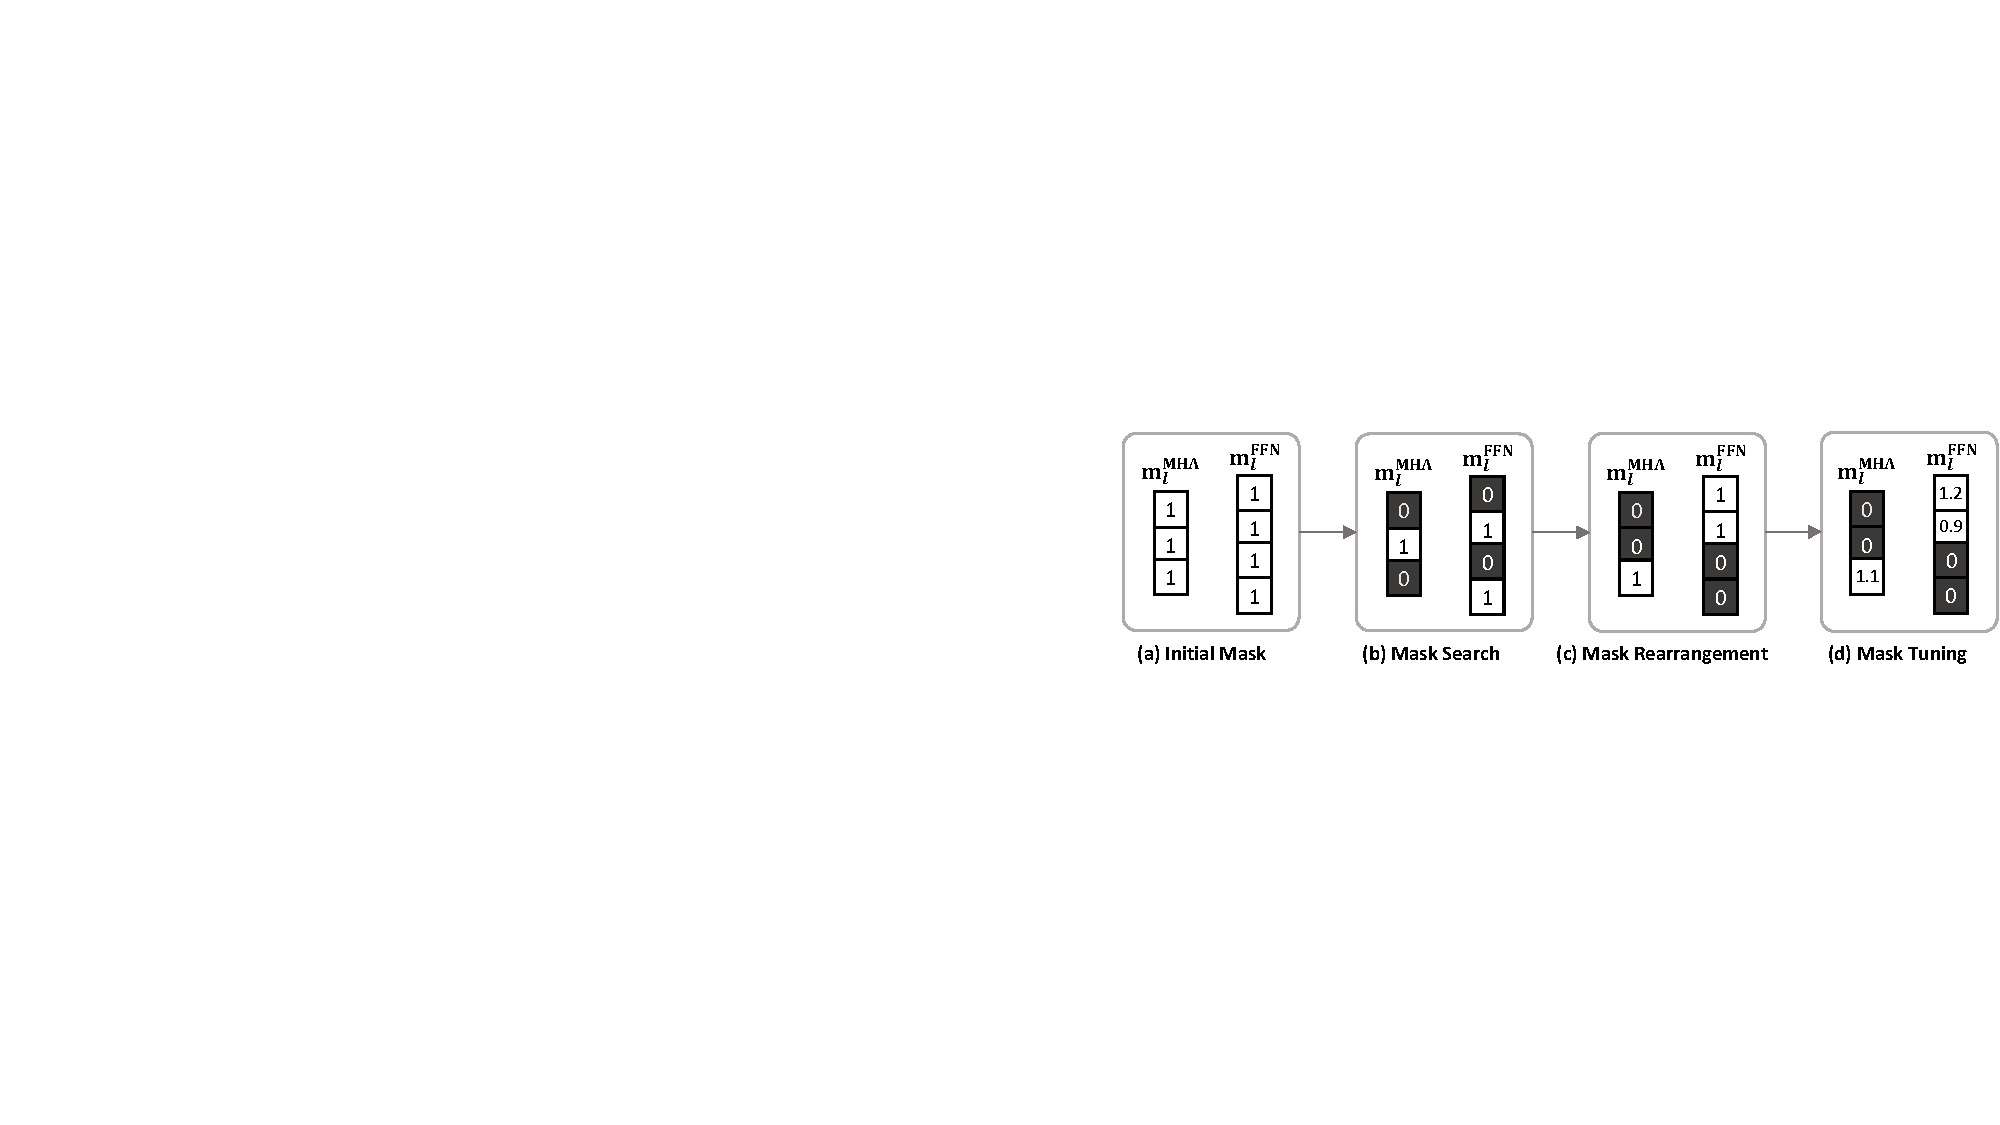
\includegraphics[width=0.75\textwidth]{figures/procedure.pdf}
    }
\caption{
Overview of our pruning framework.
(a) The mask variables 
are initialized as 1.
Then they undergo the three-stage pipeline of (b) mask search (\sref{subsec:search}), (c) rearrangement (\sref{subsec:rearrange}), and (d) tuning (\sref{subsec:tuning}).
}
\vspace{-4mm}
\label{fig:procedure}
\end{figure}
%%%%%%%%%%%%%%%%%%%%%%%%%%%%%%%%%%%%%%%%%%%%%%%%%%%%%

\vspace{-1mm}
\subsection{Framework Overview}
\label{subsec:overview}

\fref{fig:overview}(b) and~\fref{fig:procedure} illustrate the overview of our framework.

\textbf{Inputs.}
Our framework has 3 inputs: a Transformer model; a sample dataset; and a resource constraint.
The input Transformer model should contain weights fine-tuned for a downstream task.
The sample dataset is a small partition of the training dataset (typically 1--2K examples) for the downstream task.
The resource constraint can be given either as the number of floating point operations (FLOPs) or as an actual latency on target hardware.
%When the resource constraint is given in terms of latency,
In the later case, we further assume that a latency lookup table for the target hardware is provided.

\textbf{Compression Pipeline.}
As illustrated in \fref{fig:procedure},
our framework consists of 3 stages: Fisher-based mask search; Fisher-based mask rearrangement; and mask tuning.
During the \textit{Fisher-based mask search }stage (\sref{subsec:search}), we search for a binary mask applied to the heads and filters based on the Fisher information of the mask variables.
Intuitively, the mask variables with relatively higher Fisher information are considered more important, and they should be less likely to be pruned~\cite{lecun1990optimal,liu2021group,molchanov2019importance}.
As finding the optimal mask that minimizes the Fisher information loss is intractable due to the large size of the full Fisher matrix,
we propose a lightweight search algorithm that finds the optimal mask under reasonable approximations.
Second, in the \textit{Fisher-based mask rearrangement} stage (\sref{subsec:rearrange}), the framework adjusts the searched mask patterns to better take into account the intra-layer interactions between the mask variables. 
Lastly, in the \textit{mask tuning} stage (\sref{subsec:tuning}), the framework tunes the nonzero mask variables to recover the accuracy drop by reconstructing the layer-wise output signal.
